\begin{minipage}{\textwidth}
\centering
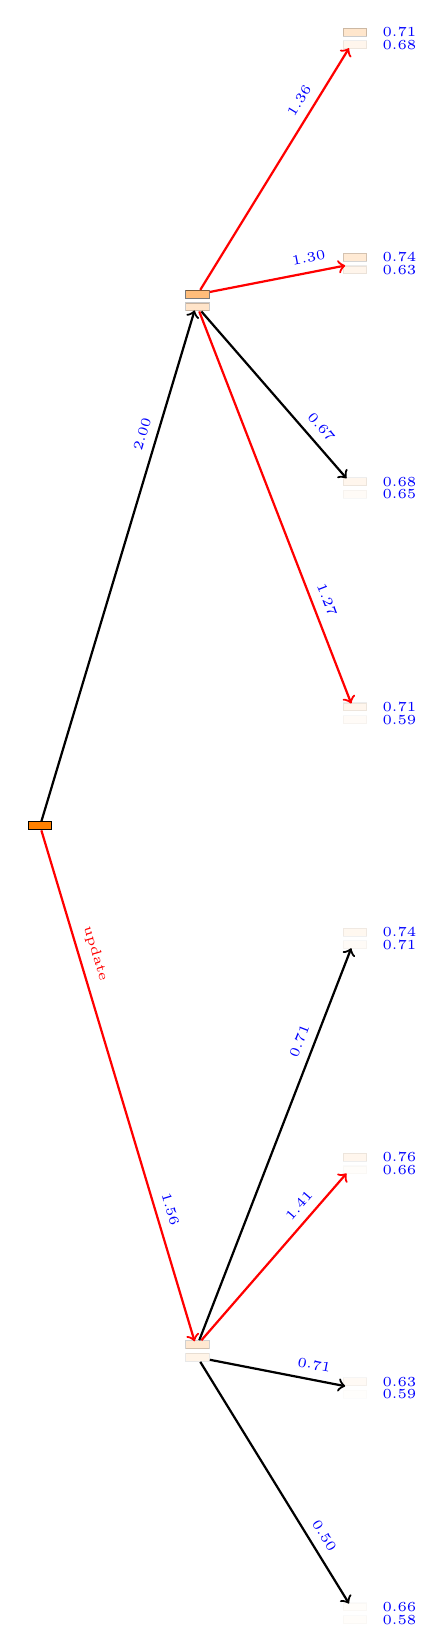
\begin{tikzpicture}
\tikzstyle{between} = [rectangle, draw=none]
\tikzstyle{state}   = [rectangle, text centered, draw=black, minimum height=1mm, text width=3mm, inner sep=0pt, fill=orange, opacity=0.2]
\tikzstyle{qval}    = [rectangle, text centered, draw=none, minimum height=1mm, text width=3mm, inner sep=0pt, fill=none]
\node[between] at (-7.00, 6.67) (1_b_0){};
\node[between] at (-7.00, -6.67) (1_b_1){};
\node[between] at (-5.00, 10.00) (2_b_0){};
\node[between] at (-5.00, 7.14) (2_b_1){};
\node[between] at (-5.00, 4.29) (2_b_2){};
\node[between] at (-5.00, 1.43) (2_b_3){};
\node[between] at (-5.00, -1.43) (2_b_4){};
\node[between] at (-5.00, -4.29) (2_b_5){};
\node[between] at (-5.00, -7.14) (2_b_6){};
\node[between] at (-5.00, -10.00) (2_b_7){};
\node[rectangle, text centered, draw=black, minimum height=1mm, text width=3mm, inner sep=0pt, fill=orange, opacity=1.00] at (-9.00, 0.00) (0_s_0){};
\node[rectangle, text centered, draw=black, minimum height=1mm, text width=3mm, inner sep=0pt, fill=orange, opacity=0.52] at (-7.00, 6.75) (1_s_0) {};
\node[rectangle, text centered, draw=black, minimum height=1mm, text width=3mm, inner sep=0pt, fill=orange, opacity=0.21] at (-7.00, 6.59) (1_s_1) {};
\node[rectangle, text centered, draw=black, minimum height=1mm, text width=3mm, inner sep=0pt, fill=orange, opacity=0.18] at (-7.00, -6.59) (1_s_2) {};
\node[rectangle, text centered, draw=black, minimum height=1mm, text width=3mm, inner sep=0pt, fill=orange, opacity=0.09] at (-7.00, -6.75) (1_s_3) {};
\node[rectangle, text centered, draw=black, minimum height=1mm, text width=3mm, inner sep=0pt, fill=orange, opacity=0.20] at (-5.00, 10.08) (2_s_0) {};
\node[qval] at (-4.50, 10.08) () {\tiny \textcolor{blue}{0.71}};
\node[rectangle, text centered, draw=black, minimum height=1mm, text width=3mm, inner sep=0pt, fill=orange, opacity=0.07] at (-5.00, 9.92) (2_s_1) {};
\node[qval] at (-4.50, 9.92) () {\tiny \textcolor{blue}{0.68}};
\node[rectangle, text centered, draw=black, minimum height=1mm, text width=3mm, inner sep=0pt, fill=orange, opacity=0.17] at (-5.00, 7.22) (2_s_2) {};
\node[qval] at (-4.50, 7.22) () {\tiny \textcolor{blue}{0.74}};
\node[rectangle, text centered, draw=black, minimum height=1mm, text width=3mm, inner sep=0pt, fill=orange, opacity=0.08] at (-5.00, 7.06) (2_s_3) {};
\node[qval] at (-4.50, 7.06) () {\tiny \textcolor{blue}{0.63}};
\node[rectangle, text centered, draw=black, minimum height=1mm, text width=3mm, inner sep=0pt, fill=orange, opacity=0.07] at (-5.00, 4.37) (2_s_4) {};
\node[qval] at (-4.50, 4.37) () {\tiny \textcolor{blue}{0.68}};
\node[rectangle, text centered, draw=black, minimum height=1mm, text width=3mm, inner sep=0pt, fill=orange, opacity=0.03] at (-5.00, 4.21) (2_s_5) {};
\node[qval] at (-4.50, 4.21) () {\tiny \textcolor{blue}{0.65}};
\node[rectangle, text centered, draw=black, minimum height=1mm, text width=3mm, inner sep=0pt, fill=orange, opacity=0.07] at (-5.00, 1.51) (2_s_6) {};
\node[qval] at (-4.50, 1.51) () {\tiny \textcolor{blue}{0.71}};
\node[rectangle, text centered, draw=black, minimum height=1mm, text width=3mm, inner sep=0pt, fill=orange, opacity=0.03] at (-5.00, 1.35) (2_s_7) {};
\node[qval] at (-4.50, 1.35) () {\tiny \textcolor{blue}{0.59}};
\node[rectangle, text centered, draw=black, minimum height=1mm, text width=3mm, inner sep=0pt, fill=orange, opacity=0.06] at (-5.00, -1.35) (2_s_8) {};
\node[qval] at (-4.50, -1.35) () {\tiny \textcolor{blue}{0.74}};
\node[rectangle, text centered, draw=black, minimum height=1mm, text width=3mm, inner sep=0pt, fill=orange, opacity=0.03] at (-5.00, -1.51) (2_s_9) {};
\node[qval] at (-4.50, -1.51) () {\tiny \textcolor{blue}{0.71}};
\node[rectangle, text centered, draw=black, minimum height=1mm, text width=3mm, inner sep=0pt, fill=orange, opacity=0.07] at (-5.00, -4.21) (2_s_10) {};
\node[qval] at (-4.50, -4.21) () {\tiny \textcolor{blue}{0.76}};
\node[rectangle, text centered, draw=black, minimum height=1mm, text width=3mm, inner sep=0pt, fill=orange, opacity=0.02] at (-5.00, -4.37) (2_s_11) {};
\node[qval] at (-4.50, -4.37) () {\tiny \textcolor{blue}{0.66}};
\node[rectangle, text centered, draw=black, minimum height=1mm, text width=3mm, inner sep=0pt, fill=orange, opacity=0.04] at (-5.00, -7.06) (2_s_12) {};
\node[qval] at (-4.50, -7.06) () {\tiny \textcolor{blue}{0.63}};
\node[rectangle, text centered, draw=black, minimum height=1mm, text width=3mm, inner sep=0pt, fill=orange, opacity=0.01] at (-5.00, -7.22) (2_s_13) {};
\node[qval] at (-4.50, -7.22) () {\tiny \textcolor{blue}{0.59}};
\node[rectangle, text centered, draw=black, minimum height=1mm, text width=3mm, inner sep=0pt, fill=orange, opacity=0.02] at (-5.00, -9.92) (2_s_14) {};
\node[qval] at (-4.50, -9.92) () {\tiny \textcolor{blue}{0.66}};
\node[rectangle, text centered, draw=black, minimum height=1mm, text width=3mm, inner sep=0pt, fill=orange, opacity=0.02] at (-5.00, -10.08) (2_s_15) {};
\node[qval] at (-4.50, -10.08) () {\tiny \textcolor{blue}{0.58}};
\draw[->, thick, black] (0_s_0) -- (1_b_0) node [near end, above, sloped, font=\tiny] () {\textcolor{blue}{2.00}};
\draw[->, thick, red] (0_s_0) -- (1_b_1) node [near start, above, sloped, font=\tiny] () {\textcolor{red}{update}} node [near end, above, sloped, font=\tiny] () {\textcolor{blue}{1.56}};
\draw[->, thick, red] (1_s_0) -- (2_b_0) node [near end, above, sloped, font=\tiny] () {\textcolor{blue}{1.36}};
\draw[->, thick, red] (1_s_0) -- (2_b_1) node [near end, above, sloped, font=\tiny] () {\textcolor{blue}{1.30}};
\draw[->, thick, black] (1_s_1) -- (2_b_2) node [near end, above, sloped, font=\tiny] () {\textcolor{blue}{0.67}};
\draw[->, thick, red] (1_s_1) -- (2_b_3) node [near end, above, sloped, font=\tiny] () {\textcolor{blue}{1.27}};
\draw[->, thick, black] (1_s_2) -- (2_b_4) node [near end, above, sloped, font=\tiny] () {\textcolor{blue}{0.71}};
\draw[->, thick, red] (1_s_2) -- (2_b_5) node [near end, above, sloped, font=\tiny] () {\textcolor{blue}{1.41}};
\draw[->, thick, black] (1_s_3) -- (2_b_6) node [near end, above, sloped, font=\tiny] () {\textcolor{blue}{0.71}};
\draw[->, thick, black] (1_s_3) -- (2_b_7) node [near end, above, sloped, font=\tiny] () {\textcolor{blue}{0.50}};
\end{tikzpicture}
\end{minipage}
